\section{Tables and Figures}

\subsection{Tables}

\begin{frame}
\frametitle{A Simple Table}
\begin{tabular}{ rlc }
	c00 & c01 & c02 \\
	c10 & c11 & c12 \\
\end{tabular}
\end{frame}


\begin{frame}
\frametitle{Borders And Alignment}
\begin{tabular}{ l | r | }
  \hline			
  This column aligns left & This column aligns right \\
  \hline			
  left & right \\
  \hline			
\end{tabular}
\end{frame}


\begin{frame}
\frametitle{Caption and Layout}
\begin{table}
\centering
\begin{tabular}{ c|c }
    left & right \\
    \hline
    left & right \\
\end{tabular}
\caption{A Sample Table}
\end{table}
\end{frame}


\subsection{Figures}


\begin{frame}{A Simple Figure}
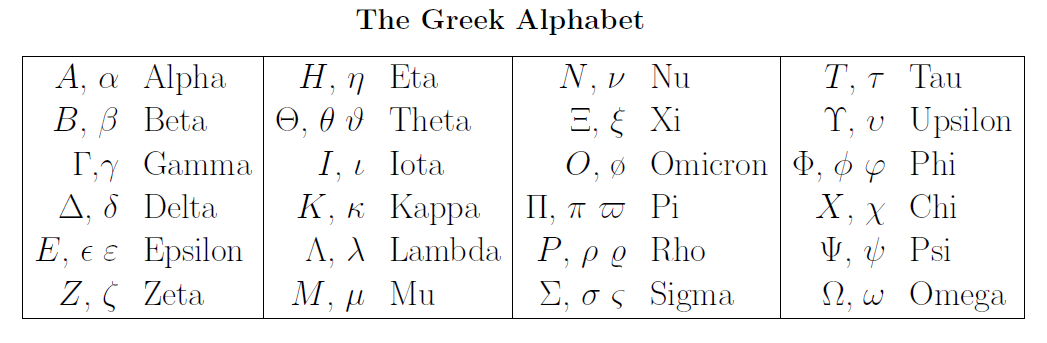
\includegraphics[width=\textwidth]{assets/greek.png}
\end{frame}


\begin{frame}{Figure in Side}
\begin{columns}

\column{.4\textwidth}
\begin{itemize}
\item Greek letters are widely used in Math
\item \lstinline|\\omega| renders $\omega$
\item \lstinline|\\Omega| renders $\Omega$
\end{itemize}

\column{.6\textwidth}
\begin{figure}[!h]
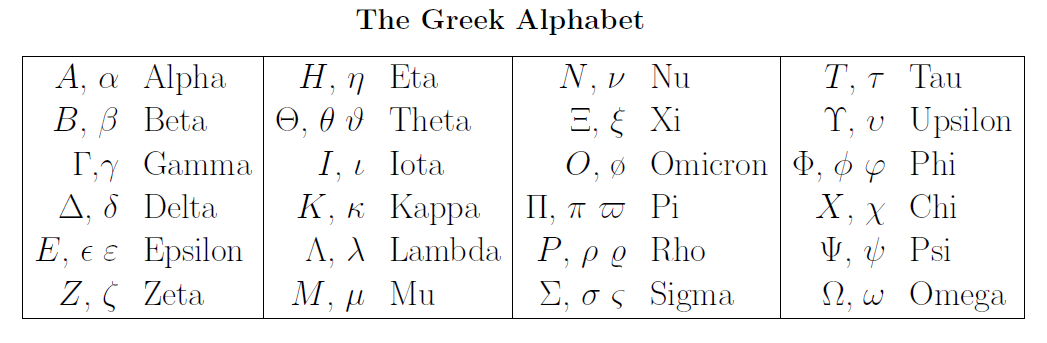
\includegraphics[width=\textwidth]{assets/greek.png}
\caption{http://3.bp.blogspot.com/-oDZ8u5SskBc/TcBKpyJyooI/AAAAAAAAABY/-AmQtxHVE5E/s1600/greek.PNG}
\end{figure}

\end{columns}
\end{frame}

